\begin{figure}[h]
    \centering
    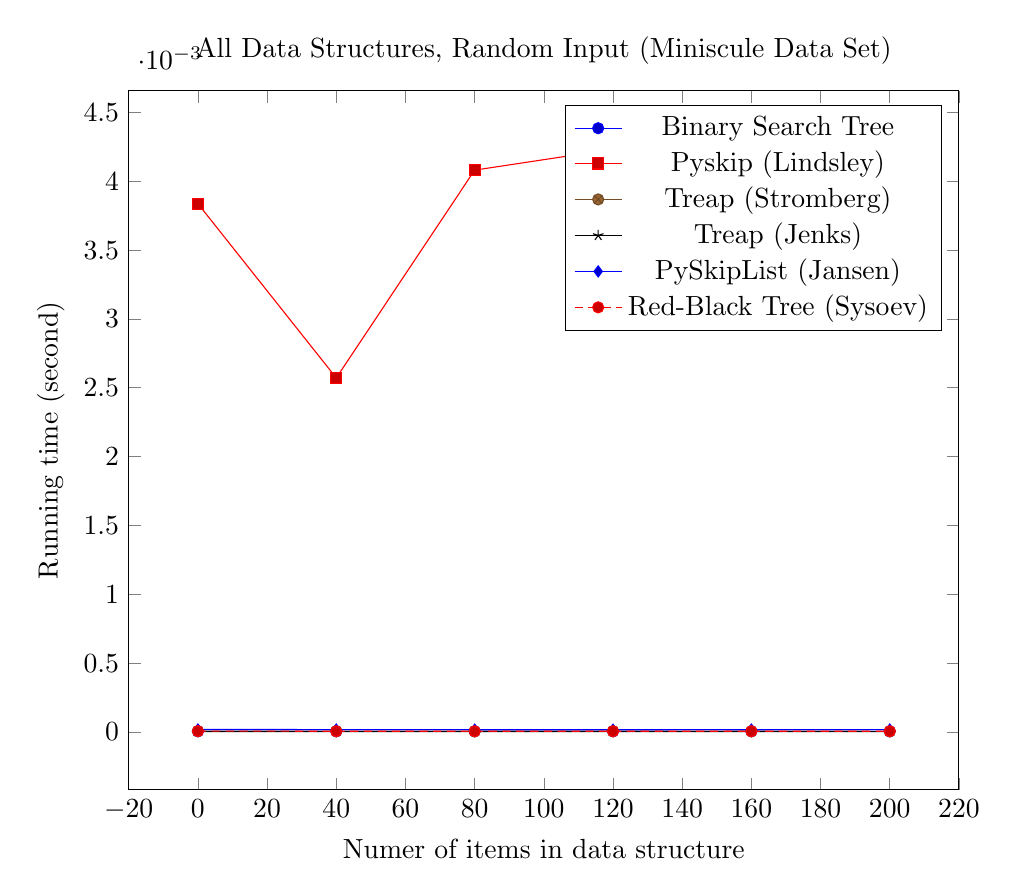
\begin{tikzpicture}
        \begin{axis}[
            xlabel={Numer of items in data structure},
            ylabel={Running time (second)},
            title={All Data Structures, Random Input (Miniscule Data Set)},
            width=\textwidth
        ]
		\addplot coordinates {
			(0, 4.367042382913411e-06)
			(40, 4.306807315557215e-06)
			(80, 4.367042382891206e-06)
			(120, 4.4875125175813935e-06)
			(160, 4.668217719649981e-06)
			(200, 4.367042382891206e-06)
		};
		\addplot coordinates {
			(0, 0.0038372448480193944)
			(40, 0.002571374790118419)
			(80, 0.0040806246376484225)
			(120, 0.0042327784177753625)
			(160, 0.004225098446688192)
			(200, 0.0038039950908419938)
		};
		\addplot coordinates {
			(0, 5.812683999284474e-06)
			(40, 6.023506735042261e-06)
			(80, 4.969393056386551e-06)
			(120, 6.17409440337724e-06)
			(160, 5.119980724765938e-06)
			(200, 4.547747584959794e-06)
		};
		\addplot coordinates {
			(0, 2.8310481654525432e-06)
			(40, 2.3190500929803904e-06)
			(80, 2.1383448909340075e-06)
			(120, 2.349167626691795e-06)
			(160, 2.0781098236000163e-06)
			(200, 2.1383448909340075e-06)
		};
		\addplot coordinates {
			(0, 1.7648874733655617e-05)
			(40, 1.722722926222886e-05)
			(80, 1.629358571828554e-05)
			(120, 1.584182271314738e-05)
			(160, 1.6986288992804076e-05)
			(200, 1.7257346795895855e-05)
		};
		\addplot coordinates {
			(0, 6.113859336043248e-06)
			(40, 5.059745657431947e-06)
			(80, 4.607982652293785e-06)
			(120, 5.059745657431947e-06)
			(160, 5.089863191098942e-06)
			(200, 5.119980724765938e-06)
		};
        \legend{Binary Search Tree, Pyskip (Lindsley), Treap (Stromberg), Treap (Jenks), PySkipList (Jansen), Red-Black Tree (Sysoev)}
        \end{axis}
    \end{tikzpicture}
    \caption{Average of 10 operations, benchmarked every 40, starting at 0.}
\end{figure}